\documentclass[11pt]{article}
\usepackage{amsmath,amssymb}
\usepackage[margin=1in]{geometry}
\usepackage{booktabs}
\usepackage{enumitem}
\usepackage{graphicx}

\begin{document}

\title{Assignment 4 Solutions}
\author{}
\date{}
\maketitle

\section*{Problem 1}

Given:
\[
\hat Y=62.4+3.57X,\qquad b_1=3.5702,\qquad s\{b_1\}=0.3470
\]
\[
n=25,\qquad df=n-2=23,\qquad s=48.82
\]

\subsection*{1(a) Test whether \(\beta_1=3.0\)}

\paragraph{Hypotheses}
\[
H_0:\beta_1=3.0
\]
\[
H_1:\beta_1\ne 3.0
\]

Use \(\alpha=0.05\), two-sided.

\paragraph{Decision rule}
Reject \(H_0\) if
\[
|t^*|>t_{0.975,23}.
\]

\paragraph{Conclusion}
\[
t^*=\frac{b_1-3.0}{s\{b_1\}}
=\frac{3.5702-3.0}{0.3470}
\approx 1.643
< t_{0.975,23}\approx 2.0687.
\]

We fail to reject \(H_0\).

\subsection*{1(b) Power if the true slope is \(3.5\)}

The consultant's standard is exceeded by \(0.5\) hour, so
\[
\beta_1=3.5.
\]
Assume
\[
\sigma\{b_1\}=0.35.
\]

The test rejects \(H_0:\beta_1=3.0\) if
\[
\left|\frac{b_1-3.0}{0.35}\right|>2.0687.
\]

Under \(\beta_1=3.5\),
\[
\frac{b_1-3.0}{0.35}\sim N\left(\frac{3.5-3.0}{0.35},1\right)
=N(1.4286,1).
\]

Thus
\[
\text{Power}
=P(T>2.0687)+P(T<-2.0687),
\quad T\sim N(1.4286,1).
\]

Approximately,
\[
\text{Power}
=P(Z>2.0687-1.4286)+P(Z<-2.0687-1.4286)
\]
\[
=P(Z>0.6401)+P(Z<-3.4973)
\approx 0.261+0.0002
\approx 0.26.
\]

So the power is about \(26\%\).

\subsection*{1(c) Why \(F^*=105.88\) is not relevant}

Because the \(F\) test is for \(H_0:\beta_1=0\) versus \(H_1:\beta_1\ne 0\), which is not the same as testing \(\beta_1=3.0\).
Perhaps we need a non-central \(F\) test.

\section*{Problem 2}
\subsection*{a.}
\[
\hat Y=156.3466-1.1900X
\]
\begin{center}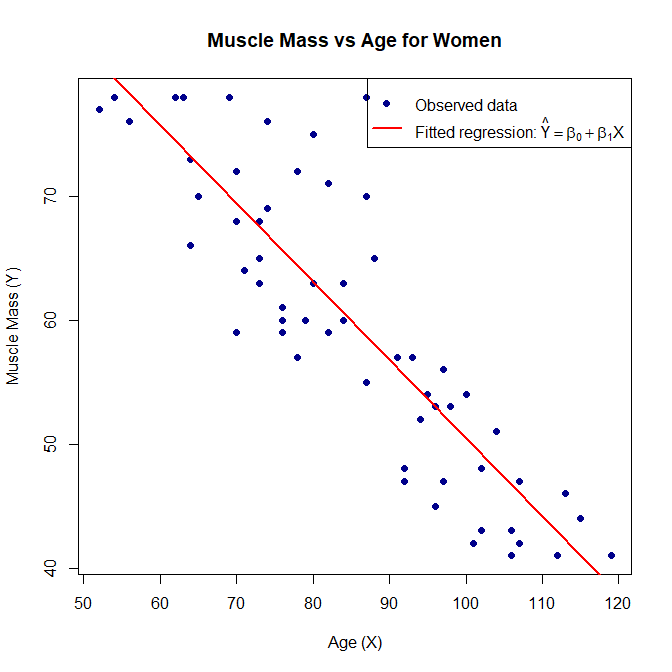
\includegraphics[width=0.8\linewidth]{p2.png}\end{center}
The plot shows a clear negative linear trend; the linear fit appears good and supports decreasing muscle mass with age.
\subsection*{b.}
\[
\hat\beta_1=-1.1900,\qquad \hat Y(60)=84.9468,\qquad e_8=4.4433,\qquad \hat\sigma^2=MSE=66.8008
\]

\section*{Problem 3}
\[
s=8.1732,\qquad t_{0.975,58}=2.0017,\qquad W=\sqrt{2F_{0.95,2,58}}=2.5127
\]
\[
\text{95\% CI for mean at }X=60:\quad (82.8346,\ 87.0590)
\]
\[
\text{95\% PI for individual at }X=60:\quad (68.4507,\ 101.4430)
\]
It is relatively precise.
\[
\text{95\% confidence band at }X=60:\quad (82.2954,\ 87.5982)
\]
The band is wider than the CI in part (a); yes, it should be wider.

\section*{Problem 4}
\subsection*{a.}
\begin{center}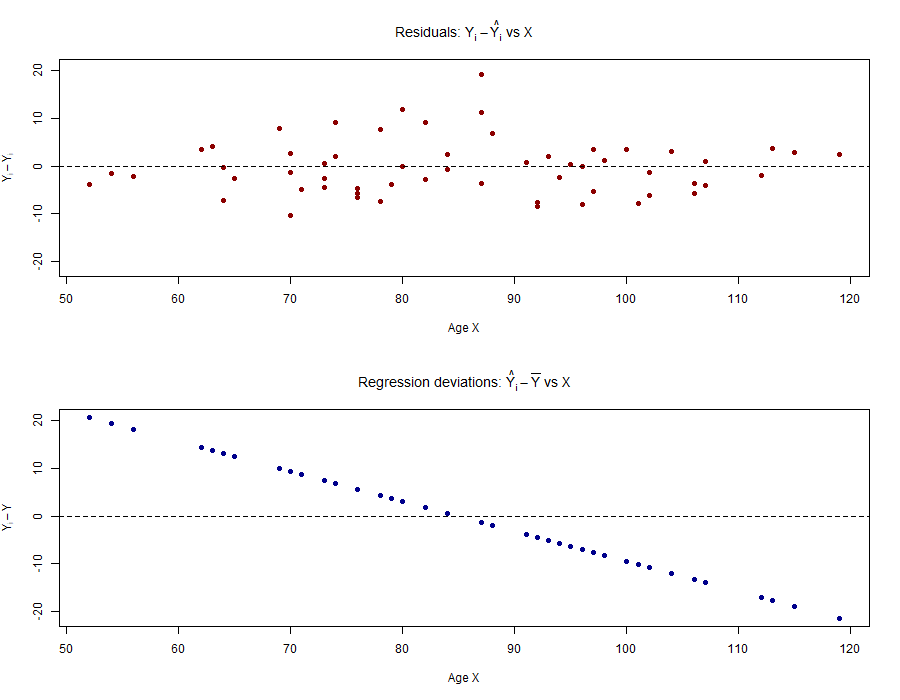
\includegraphics[width=0.8\linewidth]{p4.png}\end{center}
Since \(SSR\) appears larger, \(R^2\) is relatively large.
\subsection*{b.}
\[
\begin{array}{l|ccc}
\text{Source} & df & SS & MS\\ \hline
\text{Regression} & 1 & 11627.4858 & 11627.4858\\
\text{Error} & 58 & 3874.4475 & 66.8008\\
\text{Total} & 59 & 15501.9333 &
\end{array}
\]
\subsection*{c.}
\[
H_0:\beta_1=0,\qquad H_1:\beta_1\ne0,\qquad F^*=174.06>F_{0.95,1,58}=4.0069
\]
Reject \(H_0\). Age is linearly related to muscle mass.
\subsection*{d.\&e.}
\[
R^2=0.7501,\qquad r=-0.8661,\qquad 1-R^2=0.2499
\]
About \(25\%\) of the total variation in muscle mass remains unexplained. It is relatively small, so the linear model is a good fit.

\section*{Problem 5}

Given:
\[
X=1,4,10,11,14,
\]
\[
\sigma=0.6,\qquad \beta_0=5,\qquad \beta_1=3.
\]

So
\[
\sigma^2=0.36.
\]

\subsection*{5(a) Expected values of \(MSR\) and \(MSE\)}

For simple linear regression,
\[
E(MSE)=\sigma^2=0.36.
\]
\[
E(MSR)=\sigma^2+\beta_1^2 S_{XX}=0.36+3^2(114)
=0.36+9(114)
=0.36+1026
=1026.36.
\]

\subsection*{5(b) Better design for detecting a regression relation}

Alternative design:
\[
X=6,7,8,9,10.
\]
Then
\[
E(MSR)=0.36+9(10)=90.36.
\]

For testing whether a regression relation exists, a larger \(S_{XX}\) gives a larger expected \(MSR\) thus a smaller \(F\), so the original design is better for detecting a nonzero slope. It spreads the \(X\) values out more.

If the principal purpose is to estimate the mean response at \(X=8\), then both designs have \(\bar X=8\), so the variance of \(\hat Y\) at \(X=8\) is
\[
\operatorname{Var}(\hat Y_h)
=
\sigma^2\left[
\frac{1}{n}
+
\frac{(X_h-\bar X)^2}{S_{XX}}
\right]
=
\frac{\sigma^2}{n}
=
\frac{0.36}{5}
=
0.072.
\]
Thus the precision at \(X=8\) is the same for both designs.

\section*{Problem 6}
\[
\sum (Y_i-\bar Y)^2
=(n-1)\sigma^2+\beta_1^2\sum (X_i-\bar X)^2
\]
The deduction in the picture misses the latter term.
\end{document}